%!TEX root = main.tex

\section{The Geometric point of view}

\begin{frame}
  \frametitle{Lattices !}
\begin{figure}
\includegraphics{tikz_lattice.pdf}
\end{figure}
\begin{definition}
  A lattice $L$ is a discrete subgroup of a finite-dimensional Euclidean vector space.
\end{definition}
\end{frame}

\begin{frame}
\frametitle{Bases of a Lattice}
\includegraphics{tikz_goodbadbasis.pdf}
\\
\begin{tabular}{cccll}
 $\bblue{\vec G}$ & $ \rightarrow$ & $\rred{\vec B}$& : easy &(randomization); \\
 $\rred{\vec B}$ & $\rightarrow$ & $\bblue{\vec G}$& : hard &(LLL, BKZ, Lattice Sieve...).
\end{tabular}
\end{frame}


\begin{frame}
  \frametitle{An important invariant: the Volume}

For any two bases $\bblue{\vec G}, \rred{\vec B}$ of the same lattice $\Lambda$:
\[ \det(\bblue{\vec G}\bblue{\vec G}^t) = \det(\rred{\vec B}\rred{\vec B}^t).\]
We can therefore define:
\[ \vol(\Lambda) = \sqrt{\det(\bblue{\vec G}\bblue{\vec G}^t)}.\]
Geometrically: the volume of any {\bf fundamental domain of $\Lambda$}. \\
\pause
\begin{alertblock}{Let $\bblue{\vec G^\star}$ be the Gram-Schmidt Orthogonalization of $\bblue{\vec G}$}
$\bblue{\vec G^\star}$ is ${\bf not}$ a basis of $\Lambda$, nevertheless:
\[\vol(\Lambda) = \sqrt{\det(\bblue{\vec G^\star}\bblue{\vec G^\star}^t)} = \prod \|\bblue{\vec g_i^\star}\|.\]
\end{alertblock}
\end{frame}

\begin{frame}
  \frametitle{What is a ``Good'' basis}
Recall that, independently of the basis $\bblue{\vec G}$ it hold that:
\[\vol(\Lambda) = \prod \|\bblue{\vec g_i^\star}\|.\]

Therefore, it is somehow equivalent that
\begin{itemize}
  \item $\max_i \|\bblue{\vec g_i^\star}\|$ is small
  \item $\min_i \|\bblue{\vec g_i^\star}\|$ is large
  \item $\kappa(\bblue{\vec G}) = \min_i \|\bblue{\vec g_i^\star}\| / \max_i \|\bblue{\vec g_i^\star}\|$ is small
\end{itemize}
\pause
\begin{exampleblock}{Good basis (rule of thumb)}
\vspace{-.5cm}
  \[\kappa(\bblue{\vec G}) = \poly(d), \qquad \forall i, \|\bblue{\vec g_i^\star}\| = \poly(d) \cdot \vol(\Lambda)^{1/d}. \]
  \vspace{-.5cm}
\end{exampleblock}
\pause
\begin{alertblock}{LLL-reduced basis (rule of thumb)}
\vspace{-.5cm}
  \[\kappa(\bblue{\vec G}) \approx (1.04)^{d}, \qquad \max_i \|\bblue{\vec g_i^\star}\| \approx (1.02)^d \cdot \vol(\Lambda)^{1/d}. \]
\vspace{-.5cm}
\end{alertblock}


\end{frame}



\begin{frame}
\frametitle{Bases and Fundamental Domains}
Each basis defines a {\bf parallelepipedic tiling}.
% Les algorithmes de Babai découpent l'espace en domaines fondamentaux {\bf parallélépipédiques} selon une base donnée.
\includegraphics{tikz_goodbadtiling.pdf}
\\
{\bf Round'off Algorithm [Lenstra, Babai]}:
\begin{itemize}
  \item<2-> Given a target \ppurple{$\vec t$}
  \item<3-> Find's $\oorange{\vec v} \in L$ at the center the tile.
\end{itemize}
\end{frame}

\begin{frame}
\frametitle{Round'off Algorithm}
\begin{tabular}{ccc}
\only<1-3>{\includegraphics{tikz_ro1.pdf}}\only<4->{\includegraphics{tikz_ro4.pdf}} & \raisebox{2cm}{
$\begin{matrix}
\uncover<2->{\times {\vec B}^{-1}} \\
\longrightarrow \\
  \\
  \\
\uncover<4->{\longleftarrow} \\   
\uncover<4->{\times \vec B} \\
\end{matrix}
$}
&
\uncover<2->{\only<1-2>{\includegraphics{tikz_ro2.pdf}}\only<3->{\includegraphics{tikz_ro3.pdf}}}
\end{tabular}
\textsc{RoundOff} Algorithm [Lenstra,Babai]:
\begin{itemize}
\item<2-> Use $\vec B$ to switch to the lattice $\mathbb Z^n$ ($\times \vec B^{-1}$)
\item<3-> round each coordinate (square tiling)
\item<4-> switch back to $L$ ($\times \vec B$)
\end{itemize}
\[\uncover<2->{\oorange{\vec t'} = \vec B^{-1} \cdot \oorange{\vec t} ;} 
\quad \uncover<3->{\ppurple{\vec v'} = \lfloor \oorange{\vec t'} \rceil;}
\quad \uncover<4->{\ppurple{\vec v} = \vec B \cdot \ppurple{\vec v'}} \] 
\end{frame}


\begin{frame}
\frametitle{Nearest-Plane Algorithm}
There is a better algorithm (\textsc{NearestPlane}) based on Gram-Schmidt Orth. $\vec B^\star$ of a basis $\vec B$:

\begin{figure}
\includegraphics{tikz_goodbadNP.pdf}
\end{figure}
\begin{itemize}
  \item Worst-case distance: $\frac 1 2 \sqrt {\sum \|\vec b_i^\star\|^2}$ \hfill (Approx-CVP)
  \item Correct decoding of $\oorange{\vec t} = \ppurple{\vec v} + \vec e$ where $\vec v \in \Lambda$ if \hfill (BDD) \[\|\vec e\| \leq \min \|\vec b_i^\star\| \] 
\end{itemize}

\end{frame}

 
\begin{frame}
\frametitle{Trapdoors from Lattices ?}
With a good basis $\bblue{\vec G}$ one can solve Approx-CVP / BDD.\\
Given only a bad basis $\rred{\vec B}$, solving CVP is a {\bf hard problem}. \vspace{.4cm}\\

\includegraphics{tikz_goodbadCVP.pdf}
\vspace{.4cm}\\
Can this somehow be used as a trapdoor ?
\end{frame}


\begin{frame}
  \frametitle{Encryption from lattices (simplified)}
  Using the (second) decoding algorithm, one can recover $\vec v, \vec e$ from $\vec w = \vec v + \vec e$ when 
 \[ \|\vec e \| \leq \min \| \vec b_i^*\| \]


Fix a parameter $\eta$:
\begin{itemize}
  \item Private key: good basis $\bblue{\vec G}$ such that $\|\vec g_i^*\| \geq \eta$
  \item Public key: bad basis $\rred{\vec B}$ such that $\|\vec b_i^*\| \ll \eta$
  \item Message : $\vec m \in \Lambda = \mathcal L(\rred{\vec B}) = \mathcal L(\bblue{\vec G})$
  \item Ciphertext : $\vec c = \vec m + \vec e$, for a random error $\vec e$, $\|\vec e\| \leq \eta$
  \item Decryption : $(\vec m', \vec e) = \textsc{NearestPlane}(\vec c)$
\end{itemize}

\end{frame}




\begin{frame}
  \frametitle{Encryption from lattices}
  
Decryption : $(\vec m', \vec e) = decode(\vec c)$\\
\includegraphics{tikz_goodbadDEC.pdf}
\begin{itemize}
  \item With the good basis $\bblue{\vec G}$, $\vec m' = \vec m$
  \item With the bad basis $\rred{\vec B}$, $\vec m' \neq \vec m$ : decryption fails !
\end{itemize}

\end{frame}


\begin{frame}
\frametitle{Signatures}

{\bf Sign}
\begin{itemize}
  \item Hash the message to a random vector $\ppurple{\vec m}$.
  \item apply \textsc{NearestPlane} with a good basis $\bblue{\vec G}$: \\
    \quad find $\oorange{\vec s} \in L$ close to $\ppurple{\vec m}$ .
\end{itemize}
\vspace{.2cm}
{\bf Verify}
\begin{itemize}
  \item check that $\oorange{\vec s} \in L$ using the bad basis $\rred{\vec B}$
    \item and that $\ppurple{\vec m}$ is close to $\oorange{\vec s}$.
\end{itemize}
\vspace{.2cm}
\includegraphics{tikz_goodbadSIGN.pdf}
\end{frame}


\begin{frame}
\frametitle{A statistical attack~[NguReg06,DucNgu12]}
The difference $\vec s - \vec m$ is always inside the parallelepiped spanned by the good basis $\bblue{\vec G}$ (or its GSO $\bblue{\vec G^\star}$):
\begin{figure}
{\centering{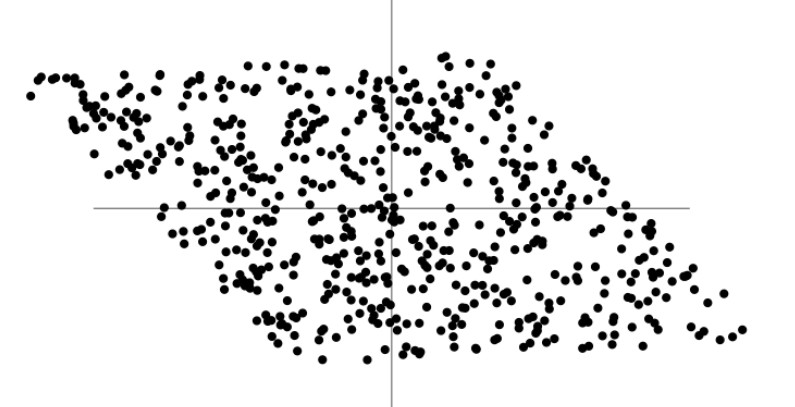
\includegraphics[width=6cm]{img/learning.jpg}}}
\end{figure}
Each signatures $(\vec s,\vec m)$ leaks a bit of information about $\bblue{\vec G}$. \\
{\bf Learning a parallepiped} from few signatures [Nguyen Regev 2006]: \\
$\quad \Rightarrow$ Total break of original GGH and NTRUSign schemes. \\
\end{frame}


\begin{frame}
\frametitle{Gaussian sampling}
Randomize the previous algorithms (Gaussian-sampling): \\
the distribution $\vec s - \vec m$ can be made {\bf independent} of $\bblue{\vec G}$
\begin{itemize}
  \item{} [Klein 2000, Gentry Peikert Vaikuthanathan 2008]: \\
  {\scriptsize Slow and memory heavy, even in the {\bf ring-setting} (NTRU, Ring-LWE)}
  \item{} [Peikert 2010] \\
  {\scriptsize Faster and less memory, but worse quality}
  \item{} [D. Prest 15] (Fast Fourier Orthogonalization) \\
  {\scriptsize Fast and good quality for certain rings}

\end{itemize}
\end{frame}
